\documentclass[11pt]{article}
\usepackage{fontspec}
\setmainfont{DejaVu Serif}
\usepackage{amsmath,amssymb}
\usepackage{geometry}\geometry{margin=2.3cm}
\usepackage{xcolor}\usepackage{graphicx}\usepackage{enumitem}\usepackage{booktabs}
\usepackage[hidelinks]{hyperref}
\definecolor{ink}{HTML}{16212e}\definecolor{accent}{HTML}{1f5fa8}\definecolor{soft}{HTML}{eef3fb}
\definecolor{warn}{HTML}{a8341f}\definecolor{good}{HTML}{16a34a}
\color{ink}
\newcommand{\key}[1]{\par\medskip\noindent\colorbox{soft}{\parbox{\dimexpr\linewidth-2\fboxsep}{\textcolor{accent}{\textbf{Κλειδί:}}\ #1}}\par\medskip}
\newcommand{\ex}[1]{\par\smallskip\noindent\textbf{\textcolor{accent}{Παράδειγμα.}}\ #1\par\smallskip}
\newcommand{\analogy}[1]{\par\smallskip\noindent\textit{\textbf{Αναλογία:}\ #1}\par\smallskip}
\newcommand{\warnb}[1]{\par\medskip\noindent\colorbox{soft}{\parbox{\dimexpr\linewidth-2\fboxsep}{\textcolor{warn}{\textbf{Προσοχή:}}\ #1}}\par\medskip}
\setlength{\parskip}{0.5em}\setlength{\parindent}{0pt}

\title{\textbf{Φροντιστήριο: Ο «κανόνας» — μια πλήρης στρατηγική trading}\\[3pt]
\large Time-series momentum + volatility targeting, βήμα-βήμα, με πραγματικά αποτελέσματα eToro\\[-1pt]
\normalsize\textcolor{accent}{momentum $\cdot$ vol-target $\cdot$ no-trade band $\cdot$ διασπορά/ENB $\cdot$ crash behavior $\cdot$ πραγματικά κέρδη}}
\author{QUANTIQ / AGEL AI --- Stefanos Drakos}\date{\today}

\begin{document}
\maketitle\thispagestyle{empty}

\noindent Αυτό το κείμενο εξηγεί από την αρχή, για αρχάριο, τη στρατηγική που στα πειράματά μας
\textbf{νίκησε κάθε μοντέλο μηχανικής μάθησης} (LSTM, transformer, gradient-boosted trees) σε πραγματικά
λεφτά: τον λεγόμενο \textbf{«κανόνα»}. Δεν έχει «μάθηση» — μόνο δοκιμασμένη λογική αγοράς. Όλα τα νούμερα
είναι από τα δικά μας πραγματικά πειράματα (paper5), και τα τελικά από \textbf{πραγματικές τιμές eToro με
πραγματικά spreads}.

\tableofcontents
\bigskip

\section{Η ιδέα σε μία πρόταση}
\textbf{«Για κάθε προϊόν: κοίτα αν ανεβαίνει ή πέφτει τους τελευταίους $\sim$6 μήνες, στοιχημάτισε προς τα
εκεί, και βάλε μέγεθος αντιστρόφως ανάλογο της μεταβλητότητάς του.»} Αυτό λέγεται \textbf{time-series
momentum με volatility targeting}.
\analogy{Σε ένα ποτάμι: κοίτα προς τα πού πάει το ρεύμα (τάση) και κολύμπα προς τα εκεί· σε ορμητικό
ποτάμι κάνε προσεκτικές, μικρές κινήσεις (μικρή θέση), σε ήρεμο κάνε μεγάλες (μεγάλη θέση).}

\section{Ο τύπος, γραμμή-γραμμή}
\begin{verbatim}
ret  = close.pct_change()                          # (1) daily returns
vol  = ret.rolling(30).std() * sqrt(252)           # (1) annualized volatility
pos  = sign(close.pct_change(120)) * (0.15/vol.shift(1))  # (2)+(3) direction x size
pos  = pos.clip(-2, 2)                             # (4) leverage cap
pos  = pos.ewm(span=5).mean()                      # (5) smoothing
pos  = apply_band(pos, 0.3)                        # (6) no-trade band
W    = pos / N                                     # (7) equal capital across products
\end{verbatim}

\subsection{(1) Μεταβλητότητα (vol) --- πόσο «τρελά» κουνιέται}
Τυπική απόκλιση των αποδόσεων 30 ημερών, ετησιοποιημένη ($\times\sqrt{252}$). Μικρή = ήρεμο, μεγάλη = άγριο.
\ex{SPY (δείκτης μετοχών) $\approx 0.15$ (15\%/έτος). BTC $\approx 0.60$ (60\%, πολύ άγριο). TLT (ομόλογα) $\approx 0.13$.}

\subsection{(2) Κατεύθυνση --- το momentum 6 μηνών}
$\mathrm{sign}(\text{απόδοση 120 ημερών})$: αν η τιμή σήμερα $>$ τιμή πριν $\sim$6 μήνες $\Rightarrow +1$
(\textbf{long}/αγορά)· αν μικρότερη $\Rightarrow -1$ (\textbf{short}/πούληση).
\key{Momentum = «ό,τι ανεβαίνει σταθερά τείνει να συνεχίσει, ό,τι πέφτει να συνεχίσει». Δοκιμασμένο εδώ
και δεκαετίες σε όλες τις αγορές.}

\subsection{(3) Μέγεθος --- το volatility targeting (ο μοχλός ρίσκου)}
Πολλαπλασιάζουμε με $0.15/\text{vol}$: διαιρώντας με τη μεταβλητότητα, παίρνουμε \textbf{μικρή θέση σε
άγριο προϊόν, μεγάλη σε ήρεμο}, ώστε κάθε στοίχημα να ρισκάρει \emph{περίπου το ίδιο} ($\sim$15\% στόχος).
Το \texttt{.shift(1)} = χθεσινή vol (αιτιατό, χωρίς να κρυφοκοιτάμε το μέλλον).
\analogy{Στο γκάζι: λίγο σε στροφές (άγριο), πολύ σε ίσιο δρόμο (ήρεμο) --- ίδιος «κίνδυνος» παντού.}
\key{Το $0.15$ είναι ο \textbf{στόχος μεταβλητότητας}: ο διακόπτης ρίσκου/κέρδους. Διπλασιάζεις $\to$
$\sim$διπλάσιο κέρδος ΚΑΙ $\sim$διπλάσιο drawdown (γραμμικά).}

\subsection{(4)--(7) Τα «φρένα» και η διασπορά}
\textbf{(4) clip $\pm2$:} όριο μόχλευσης $\pm2\times$ (να μη δώσει τρελή θέση σε υπερ-ήρεμο προϊόν).
\textbf{(5) ewm(5):} εξομάλυνση $\sim$5 ημερών $\to$ η θέση δεν χοροπηδά κάθε μέρα (λιγότερος θόρυβος).
\textbf{(6) no-trade band (0.3):} δεν αλλάζεις θέση για \emph{μικρές} κινήσεις του σήματος --- γλιτώνεις
κόστη συναλλαγών. \textbf{(7) /N:} \textbf{ισόποσα} σε όλα τα προϊόντα (διασπορά).
\analogy{Ο θερμοστάτης (band): δεν ανάβει/σβήνει το καλοριφέρ για κάθε 0.1$^\circ$C.}

\section{Αναλυτικό παράδειγμα --- μία μέρα, τρία προϊόντα}
Έστω, σήμερα:
\begin{center}\small
\begin{tabular}{lccccl}
\toprule
Προϊόν & τιμή πριν 6μ & τιμή σήμερα & τάση & vol & θέση $=\mathrm{sign}\times 0.15/\text{vol}$ \\
\midrule
BTC & 40k & 50k & $\uparrow$ ($+1$) & 0.60 & $+1\times 0.15/0.60 = \mathbf{+0.25}$ (μικρό long) \\
SPY & 480 & 520 & $\uparrow$ ($+1$) & 0.15 & $+1\times 0.15/0.15 = \mathbf{+1.00}$ (πλήρες long) \\
TLT & 95 & 88 & $\downarrow$ ($-1$) & 0.13 & $-1\times 0.15/0.13 = \mathbf{-1.15}$ (short) \\
\bottomrule
\end{tabular}
\end{center}
Μετά: clip $\pm2$ (όλα εντός), εξομάλυνση, band, και \textbf{/3} (ισόποσα). Παρατήρησε: το BTC, παρότι
ανεβαίνει, παίρνει \textbf{μικρή} θέση γιατί είναι άγριο --- το vol-targeting εξισώνει το ρίσκο.

\section{Τα εργαλεία μέτρησης που χρησιμοποιούμε}
\textbf{IR (Information Ratio)} $=\sqrt{\text{ppy}}\cdot \bar r/\sigma_r$: κέρδος ανά μονάδα ρίσκου,
ετησιοποιημένο. \emph{Δεν} είναι το \% κέρδος --- είναι η \textbf{ομαλότητα}. IR $>1$ = πολύ καλό.
\textbf{maxDD} = η χειρότερη πτώση από κορυφή (πόσο «πονάει» στο χειρότερο). \textbf{net} = κέρδος
\emph{μετά} τα κόστη: χρεώνουμε το \textbf{πραγματικό spread} κάθε προϊόντος στο turnover (eToro: BTC/ETH
$\sim$31 bps, ETF 1--4 bps). \textbf{ENB} (effective number of bets) $=(\sum\lambda)^2/\sum\lambda^2$:
πόσα \emph{πραγματικά ανεξάρτητα} στοιχήματα έχεις (αν 2 προϊόντα κινούνται μαζί, μετράνε για 1).
\textbf{Leak-free walk-forward}: εκπαιδεύεις/μετράς πάντα στο \emph{παρελθόν}, ελέγχεις στο \emph{αδίδακτο}
μέλλον --- καμία ζαβολιά.
\key{Υψηλό IR $\ne$ πολλά λεφτά. Σημαίνει \emph{σταθερό, χαμηλού-drawdown} κέρδος. Το απόλυτο \% το ορίζει
ο στόχος ρίσκου (0.15).}

\section{Τα πραγματικά κέρδη στο eToro}
Πλήρες leak-free backtest σε \textbf{πραγματικές eToro τιμές} (14 προϊόντα, 2023--2026 incl. το bear του
2022--23), με \textbf{πραγματικά per-asset spreads}:
\begin{center}\small
\begin{tabular}{llrrrr}
\toprule
μοντέλο & band & total \% & /έτος \% & IR & maxDD \\
\midrule
\textbf{κανόνας} & hard & \textbf{+28.7\%} & \textbf{+10.2\%} & \textbf{1.53} & $-6\%$ \\
κανόνας & none & +22.8\% & +8.3\% & 1.26 & $-7\%$ \\
GBT (trees) & hard & +9.6\% & +3.6\% & 1.06 & $-3\%$ \\
LSTM (deep) & hard & --- & $\sim$0\% & 1.00 & $-5\%$ \\
\bottomrule
\end{tabular}
\end{center}
\key{Σε €10.000: ο κανόνας $\to$ \textbf{€12.866} σε 2.6 χρόνια. Μέτρια αλλά \textbf{πολύ σταθερά}
(maxDD $-6\%$). Τα κέρδη κλιμακώνονται με τον στόχο ρίσκου. Ο \textbf{απλός κανόνας κερδίζει σε λεφτά ΚΑΙ
σε σταθερότητα} κάθε μοντέλο ML.}
\begin{center}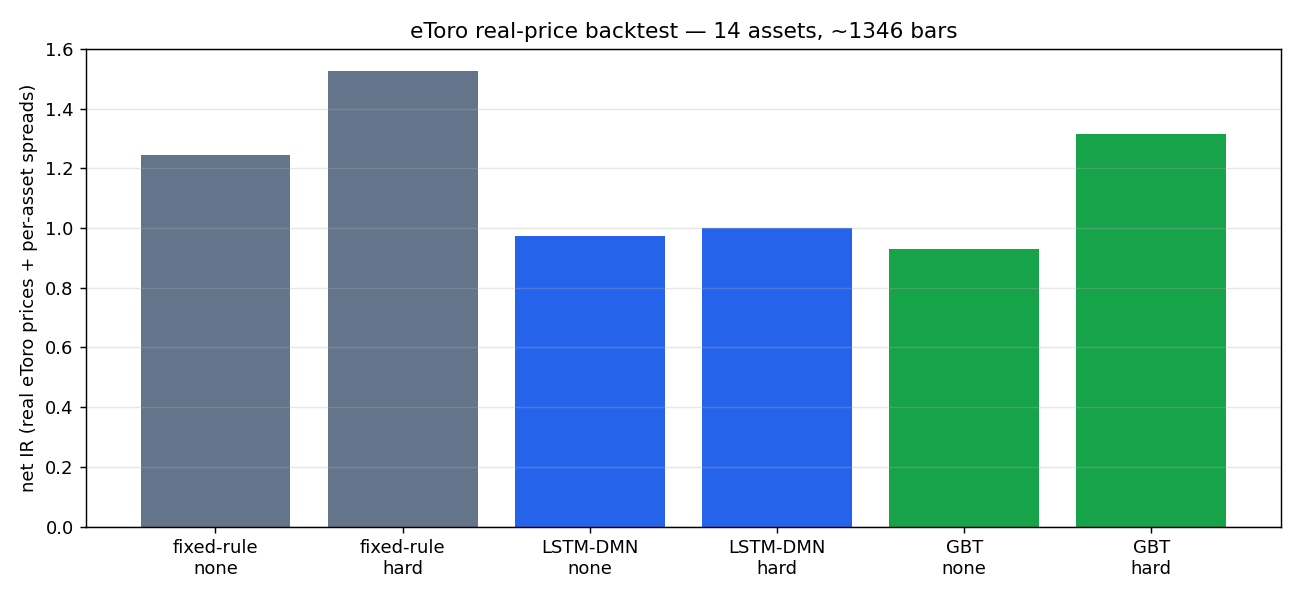
\includegraphics[width=0.92\linewidth]{figures/fig_etoro_gbt_backtest.png}\end{center}

\section{Diversity \texorpdfstring{$>$}{>} count --- το πείραμα 3 / 5 / 14 προϊόντων}
Ίδια περίοδος (2.7 χρόνια, πραγματικές eToro τιμές), ο κανόνας σε τρία baskets:
\begin{center}\small
\begin{tabular}{lcccccr}
\toprule
basket & n & ENB & total \% & /έτος \% & IR & maxDD \\
\midrule
B3 (SPY,TLT,BTC) & 3 & 3.0 & +28.6\% & +9.7\% & 1.12 & $-9\%$ \\
\textbf{B5 (+GLD,UUP)} & 5 & 4.5 & \textbf{+34.9\%} & \textbf{+11.6\%} & \textbf{1.63} & $\mathbf{-5\%}$ \\
B14 (όλα) & 14 & 6.5 & +26.9\% & +9.1\% & 1.61 & $-6\%$ \\
\bottomrule
\end{tabular}
\end{center}
\textbf{Τι μαθαίνουμε:}
\begin{itemize}[leftmargin=1.4em]
\item \textbf{Τα 5 καλο-διαλεγμένα = το γλυκό σημείο}: μεγαλύτερο κέρδος (+11.6\%/έτος), καλύτερο IR
(1.63), μικρότερο drawdown ($-5\%$). €10k $\to$ \textbf{€13.495}.
\item \textbf{3 προϊόντα}: καλά αλλά πιο \emph{τραχύ} (maxDD $-9\%$, IR 1.12) --- λίγα bets, μεγαλύτερες
ταλαντώσεις.
\item \textbf{14 προϊόντα ΔΕΝ βελτιώνουν τα 5}: το ENB είναι μόλις \textbf{6.5/14} (46\%) --- τα επιπλέον
9 (SPY/QQQ/EEM/EFA όλα μετοχές) είναι \textbf{πλεονάζοντα}.
\end{itemize}
\key{\textbf{«5 ασυσχέτιστα $>$ 14 πλεονάζοντα.»} Σημασία έχει ο αριθμός των \emph{ανεξάρτητων} bets (ENB),
όχι των ονομάτων. Η διασπορά κορεσμένει γύρω στα 5 σωστά (διαφορετικές κλάσεις: μετοχές, ομόλογα, χρυσός,
crypto, δολάριο).}

\section{Σε crash τι γίνεται;}
\textbf{Δύναμη --- μπορεί να γίνει SHORT.} Μετά από $\sim$6 μήνες πτώσης το πρόσημο γυρίζει σε $-1$ $\to$ η
στρατηγική \textbf{πουλάει} $\to$ \textbf{κερδίζει από την πτώση} («crisis alpha»). Στο παράθυρό μας που
περιλαμβάνει το bear του 2022, ο κανόνας ήταν \textbf{θετικός}.

\textbf{Αυτόματο φρένο --- vol-targeting.} Σε crash η μεταβλητότητα εκτοξεύεται $\to$ το $0.15/\text{vol}$
\textbf{μικραίνει μόνο του τη θέση} $\to$ μικρότερες ζημιές. Γι' αυτό το maxDD ήταν μόλις $-6\%$.

\warnb{Η αδυναμία --- «momentum crash»: \textbf{αστραπιαία} βουτιά + V-ανάκαμψη. Το σήμα είναι αργό (6μ).
Αν το crash γίνει σε εβδομάδες (π.χ. COVID Μάρτιος 2020) πριν γυρίσει το πρόσημο, η στρατηγική είναι ακόμα
\emph{long} και τρώει τη βουτιά· κι αν γυρίσει short στον πάτο και η αγορά αναπηδήσει, τρώει \textbf{whipsaw}
(short μέσα σε ράλι). Ο εχθρός του momentum δεν είναι οι αργές πτώσεις (τις κερδίζει) αλλά οι \textbf{απότομες
αντιστροφές}.}
Άμυνες που έχουμε: vol-targeting (auto-deleverage), band+εξομάλυνση (αποφυγή whipsaw σε θόρυβο), και
\textbf{διασπορά} (τα ομόλογα TLT συχνά ανεβαίνουν σε equity crash --- αντισταθμίζουν).

\section{Είναι αυτόνομη στρατηγική;}
\textbf{Ναι --- είναι ήδη πλήρης.} Έχει σήμα (momentum), μέγεθος (vol-target), φρένα (clip/band/ewm),
διασπορά (/N). Δεν χρειάζεται ML. Είναι \textbf{deployable ως έχει} και ο \textbf{καλύτερος σε λεφτά}.
Προϋποθέσεις: μέτριες αλλά σταθερές αποδόσεις (στο 0.15)· θέλει \textbf{$\sim$5 ασυσχέτιστα προϊόντα}
(όχι ένα όνομα)· πειθαρχία (καθημερινό rebalance + το band για κόστη).

\section{Πώς εξερευνείται παραπάνω (χωρίς περισσότερο ML)}
Οι μοχλοί είναι στο \textbf{risk management}, όχι στη χωρητικότητα μοντέλου:
\begin{center}\small
\begin{tabular}{ll}
\toprule
Κατεύθυνση & Τι κάνει \\
\midrule
Vol-target tuning & $0.15\to0.30$ = $\sim\times2$ κέρδος ΚΑΙ drawdown (ο διακόπτης ρίσκου) \\
\textbf{BOCPD changepoint φρένο} & κόβει θέσεις σε αλλαγή regime $\to$ μειώνει το momentum-crash \\
Multi-horizon (60/120/250) & μείγμα οριζόντων $\to$ πιο σταθερό σήμα \\
Fast-reversion overlay & βραχυπρόθεσμη mean-reversion ενάντια στο whipsaw \\
VIX / crisis gate & μικραίνει θέσεις όταν εκτοξεύεται ο φόβος \\
Περισσότερα ασυσχέτιστα assets & υψηλότερο ENB $\to$ ομαλότερο \\
\bottomrule
\end{tabular}
\end{center}
\key{Το πιο υποσχόμενο: \textbf{BOCPD φρένο + multi-horizon} --- χτυπούν ακριβώς την αδυναμία (απότομες
αντιστροφές) και βελτιώνουν το risk-adjusted, \textbf{χωρίς} overfit.}

\section{Γιατί ο απλός κανόνας νικά το ML}
Δοκιμάσαμε εξαντλητικά: LSTM, transformer (4 μορφές), synthetic pretraining, gradient-boosted trees.
\textbf{Κανένα deep μοντέλο δεν ξεπέρασε τον κανόνα.} Ο λόγος: ο κανόνας \textbf{κωδικοποιεί κατευθείαν}
δοκιμασμένη γνώση (momentum, μέγεθος-κατά-ρίσκο, διασπορά, έλεγχος κόστους) με \textbf{μηδέν παραμέτρους
προς μάθηση} $\to$ μηδέν overfit. Το ML έπρεπε να τα \emph{ανακαλύψει μόνο του} από λίγα/θορυβώδη δεδομένα
και δεν τα κατάφερε καλύτερα.
\key{Σε λεπτά χρηματοοικονομικά δεδομένα: \textbf{πιο απλό $>$ πιο βαθύ}. Ο κανόνας ξεκινά με τη σωστή
απάντηση· το δίκτυο πρέπει να την ψάξει --- και χάνει.}

\section{Σύνοψη}
\begin{itemize}[leftmargin=1.4em]
\item Ο κανόνας = \textbf{ακολούθησε την τάση 6μήνου, μέγεθος αντιστρόφως ανάλογο της μεταβλητότητας,
ισόποσα, με έλεγχο κόστους}.
\item Πραγματικά eToro: \textbf{+10.2\%/έτος, IR 1.53, maxDD $-6\%$} (€10k$\to$€12.866) --- νικά κάθε ML.
\item Διασπορά: \textbf{5 ασυσχέτιστα = γλυκό σημείο} (+11.6\%/έτος, IR 1.63)· περισσότερα πλεονάζοντα δεν
βοηθούν.
\item Crash: κερδίζει τις \emph{αργές} πτώσεις (short + auto-deleverage)· ευάλωτος σε \emph{απότομες}
αντιστροφές --- διορθώνεται με BOCPD φρένο.
\item Αυτόνομη, σταθερή, επεκτάσιμη --- και πιο αξιόπιστη από κάθε νευρωνικό δίκτυο εδώ.
\end{itemize}

\end{document}
